\subsection{Building the index}
	\textbf{Student Name: }Christian Stevandy \textbf{ID:} 0870945\\\\
	This section describes how the post index are build and how the post retrieved from a query in the index.
\subsubsection*{Motivation}
	User post contains a lot of interested information. People can retrieve information in a post by giving a query in our search engine. In order to answer a query from a user it is required to make index for user posts.
\subsubsection*{Problem formulation}
	Given a collection of posts in JSON representation and a query from user. The posts are used for building index. Query from user retrieves information from the index.
\subsubsection*{Approach}
	We built the index from posts that are generated by the crawler. The query is handled using boolean retrieval and vector space model representation and also created our user post database for offline use.\\\\
	\textbf{a. Building the Index} \\\\
	The index is implemented by using the library Lucene. The user posts generated by the crawler are stored in this Lucene index: \\\\\\\\\\\\\\\\
	\begin{figure}[h]
		\begin{center}
			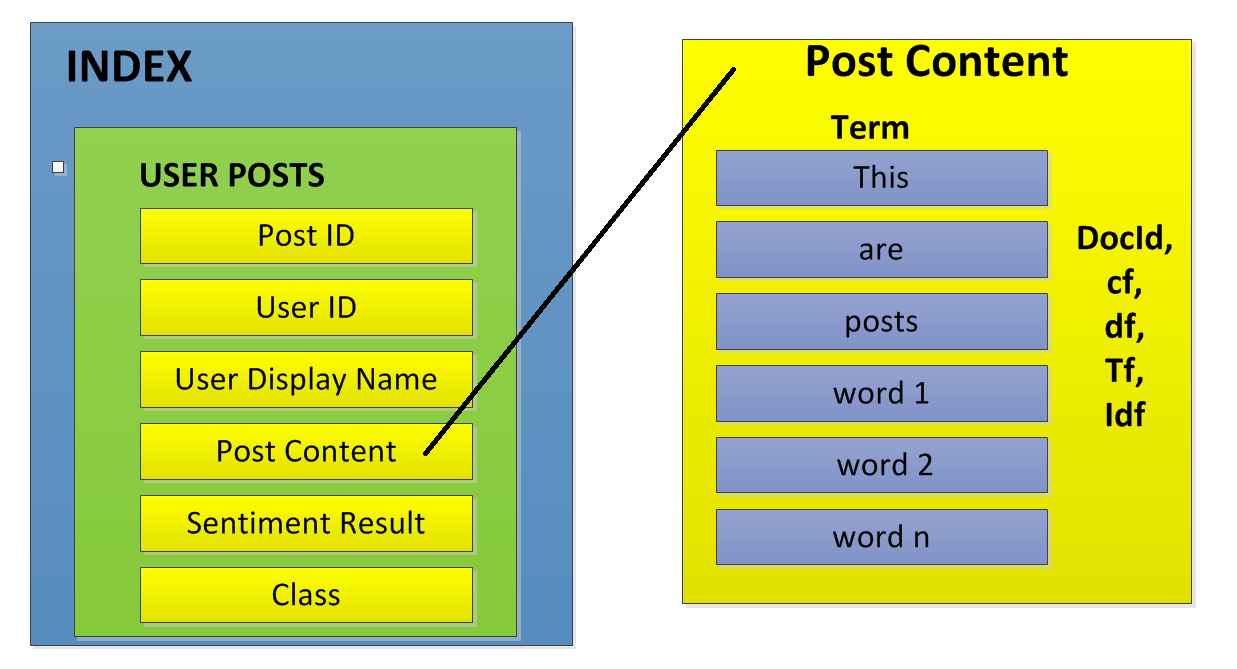
\includegraphics[scale=0.4]{images/postindex.png}
		\caption{Post Index\label{post_index}}
		\end{center}
	\end{figure}
	\\Figure~\ref{post_index} consist of multiple fields. One of its fields is Post Content, this field represent a text of a user post which is contains an inverted index and documents vector space model.\\\\
	\textbf{b. Searching Index}\\\\
	Searching is implemented using Lucene with boolean query and vector space model techniques.\\
	\\
	\textbf{Boolean Query}\\
		-  OR query is processed by unioning term’s posting list in index.\\
		-  AND query is processed by intersecting term’s posting list in index.\\
	\\
	\textbf{Scoring Document}\\
	In vector space model, user posts are represented in a collection of string vector. For example, a post ��This is a post�� will be represented as string vector (This,is,a,post).
	The retrieved user posts are ranked based on how high their score are. Score is calculated using cosine similarity in vector space model.\\
	\begin{figure}[h]
		\begin{center}
			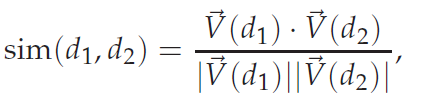
\includegraphics[scale=0.4]{images/cosinesim.png}
		\caption{Cosine Similarity Equation\label{cosinesim}}
	\end{center}
	\end{figure}

\subsubsection{Evaluation}
Evaluation is done manually by giving a query and evaluates the result. Index should be built first before testing a query. A test query is given by giving a Boolean ‘OR’, ‘AND’. The query result is listed by their rank so it is conclude this task is satisfying.

